\section{Application to Undergraduate Chemistry Laboratories}
As a proof of concept, the authors applied the thermal analysis Arduino system to an experiment currently used in an undergraduate 
General Chemistry laboratory course.  The objective of this experiment is to determine the optimal (stoichiometric) ratio of two 
reactants in a chemical reaction using the method of continuous variations~\cite{job}.  Reactants are chosen such that an 
exothermic (heat-releasing) reaction occurs; the heat released manifests as an increase in the mixture’s temperature.  
Systematically varying the ratio of these reactants and monitoring the associated temperature change ($\Delta T$) allows for the 
determination of the optimal ratio in the chemical reaction by identifying the proportion that generates the largest $\Delta T$.  
Two sets of reactants were chosen for this experiment: (1) sodium hypochlorite (NaClO) with potassium iodide (KI) and (2) NaClO with 
sodium sulfite (Na$_2$SO$_3$)~\cite{vonderbrink}.  Other combinations including 
sodium hydroxide with hydrochloric acid, 
%sodium hydroxide and 
acetic acid, 
%sodium hydroxide and 
oxalic acid,
sulfuric acid, or
phosphoric acid,
potassium hydroxide with citric acid, and sodium hypochlorite with sodium 
thiosulfate have been utilized elsewhere~\cite{mahoney,vernier,vonderbrink,tatsuoka}.

Details of the laboratory procedure can be found in Reference~\cite{vonderbink}, but 
salient details and modifications are summarized below.   0.50 M NaClO($aq$), 0.50 M KI($aq$), and 0.50 M Na$_2$SO$_3$($aq$) 
solutions were prepared.\footnote{The KI and Na$_2$SO$_3$ solutions also contained sodium hydroxide at a  0.2 M concentration.  
Details are provided in Supporting Information.}  Nine mixtures with unique ratios of each (1) NaClO solution to 
KI solution and (2) NaClO solution to Na$_2$SO$_3$ solution (by volume) were prepared such that the total volume of 
each mixture was fixed at 50.0 mL.  Components of the mixtures were kept separated until the time of the experiment.  For 
each trial, the component available in the largest volume was added to two nested Styrofoam cups and subjected to moderate magnetic stirring.  
The thermistor of the Ardunio was inserted into the liquid.  Temperature was monitored to ensure thermal equilibrium and a stable initial temperature.  
The second component was added to the first component in the cups; a button on the Arduino was pushed to record the time of mixing.  
Temperature of the resulting mixture was monitored for at least two additional minutes.  

\subsection{Determining the Optimal Ratio of the NaClO and KI Reaction}
Profiles of the observed changes in temperature with time for the reactions of NaClO and KI are shown in Figure~\ref{fig:temp_KI}.  
All temperature changes in Figure~\ref{fig:temp_KI} are expressed relative to the temperature of solution prior to mixing.  
This reference temperature for each mixture was determined as the average temperature taken over the fifteen data points prior to mixing.  
All profiles were shifted horizontally such that the time of mixing corresponds to $t = 0$ s.  Each profile is distinguished using the ratio of mL of 
NaClO($aq$) to mL of KI($aq$).

\begin{figure}[htbp]
\centering
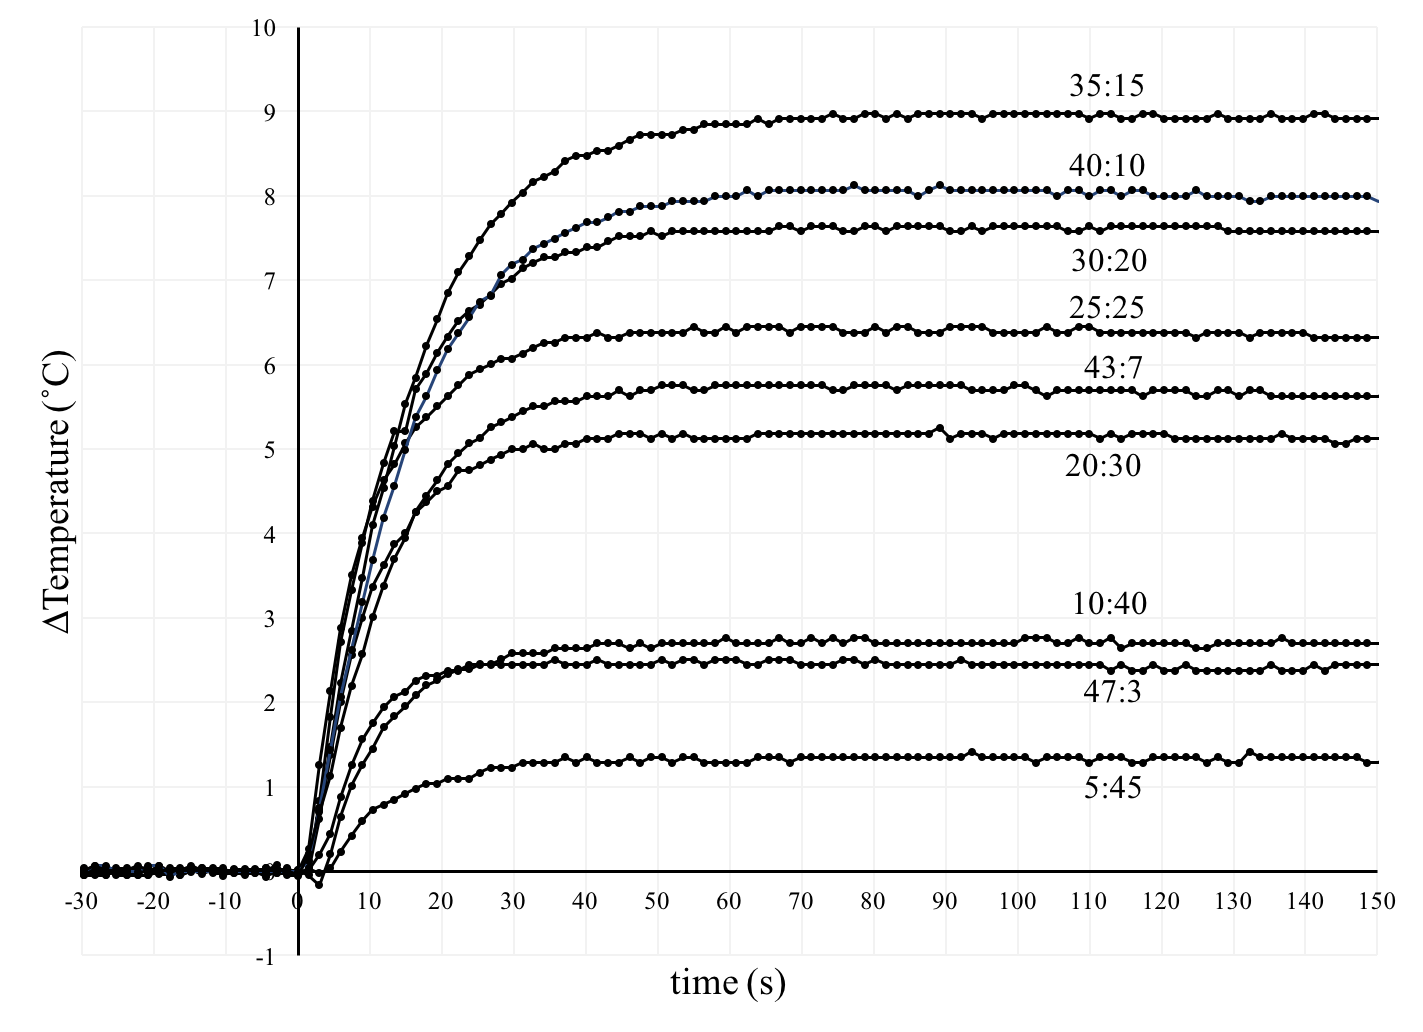
\includegraphics[width=\textwidth]{Temperature_Profiles_KI_BW.png}
\caption{Variation of Temperature with Time for Mixtures of NaClO($aq$) and KI($aq$)}
\label{fig:temp_KI}
\end{figure}


From the data sets for each trial, a maximum temperature change ($\Delta T_\mathrm{max}$) was determined.  
These $\Delta T_\mathrm{max}$ values were then plotted against the volume of NaClO solution present in the reaction 
mixture (Figure~\ref{fig:var_KI}).  In addition to the nine measured data points, two additional points 
corresponding to 0.0 mL NaClO($aq$):50.0 mL KI($aq$) and 50.0 mL NaClO($aq$):0.0 mL KI($aq$) were included.  
Since no reaction occurs at these compositions, $\Delta T_\mathrm{max}$ was taken to be 0.0$^\circ$C for these points.  
Lines of best fit through points falling on increasing and decreasing $\Delta T_\mathrm{max}$ with volume NaClO($aq$) 
trends were determined.\footnote{The upward trendline was set to include the point (0.0 mL, 0.0$^\circ$C). The downward 
trendline was set to include the point (50.0 mL, 0.0$^\circ$C). The corresponding equations were 
$\Delta T_\mathrm{max}$ = (0.2578$^\circ$C/mL) $V$ ($R^2$ = 0.99895) and $\Delta T_\mathrm{max}$ = ($-0.8169^\circ$C/mL) $V$ + 40.845$^\circ$C ($R^2$= 0.99983).}  

\begin{figure}[htbp]
\centering
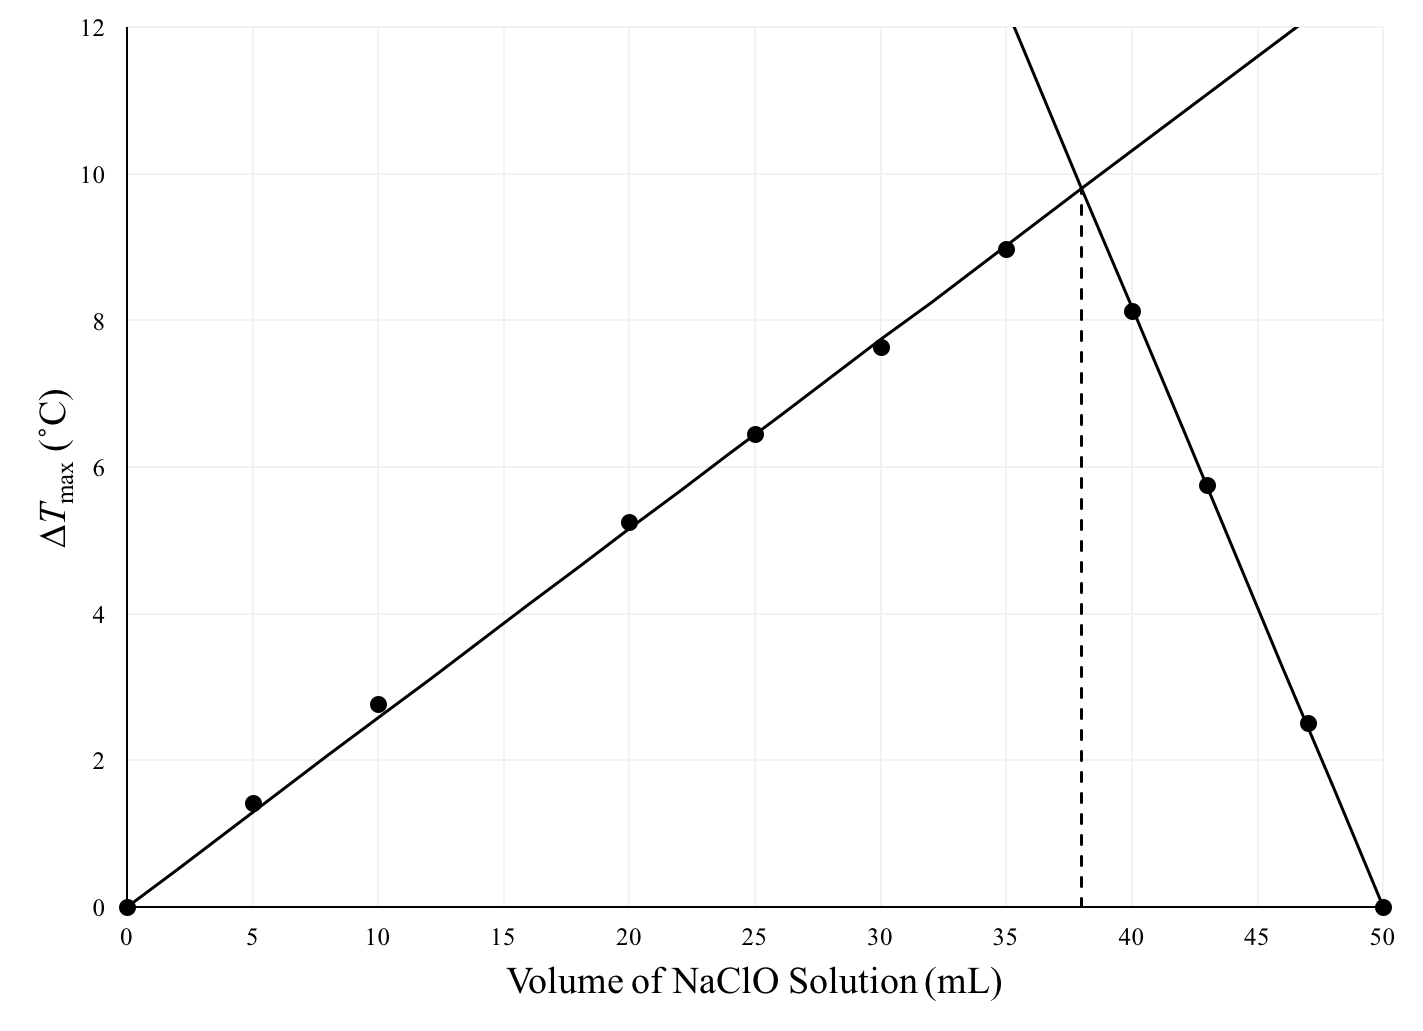
\includegraphics[width=\textwidth]{Bleach_KI_Variations_alt.png}
\caption{Maximum Temperature Changes Observed for Each Reaction Mixture of NaClO($aq$) and KI($aq$)}   %Variation of Temperature with Time for Mixtures of NaClO($aq$) and KI($aq$)}
\label{fig:var_KI}
\end{figure}

In this experimental method, the heat generated from each reaction (proportional to the $\Delta T_\mathrm{max}$ observed) 
will increase as components react more completely.  The optimal (stoichiometric) proportion of two reactants will yield the largest $\Delta T_\mathrm{max}$.  
By extrapolating the two linear trendlines to a point of intersection, we estimate the largest $\Delta T_\mathrm{max}$ to be 9.80$^\circ$C.  
This corresponds to an optimal ratio of 38.0 mL NaClO($aq$):12.0 mL KI($aq$), which is in agreement with the actual 3:1 ratio for this 
reaction.\footnote{Since solutions are at equal concentrations, the ratio of volumes is equivalent to the ratio of amounts used to establish the 
stoichiometry of the reaction.  The actual stoichiometry of 3:1 is based on the net ionic equation: 3ClO$^-$($aq$) + I$^-$($aq$) $\rightarrow$ 3Cl$^-$($aq$) + IO$_3^-$($aq$)~\cite{vonderbrink}.}

\subsection{Determining the Optimal Ratio of the NaClO and Na$_2$SO$_3$ Reaction}
The experiment was repeated using sodium hypochlorite (NaClO) with %a different reactant, 
sodium sulfite (Na$_2$SO$_3$).  
Temperature versus time plots for the NaClO and Na$_2$SO$_3$ reactions are shown in Figure~\ref{fig:temp_Na2SO3}.  
All temperature changes are expressed relative to the pre-mixing temperature and times are expressed relative to 
the time of mixing, as discussed previously.  

\begin{figure}[htbp]
\centering
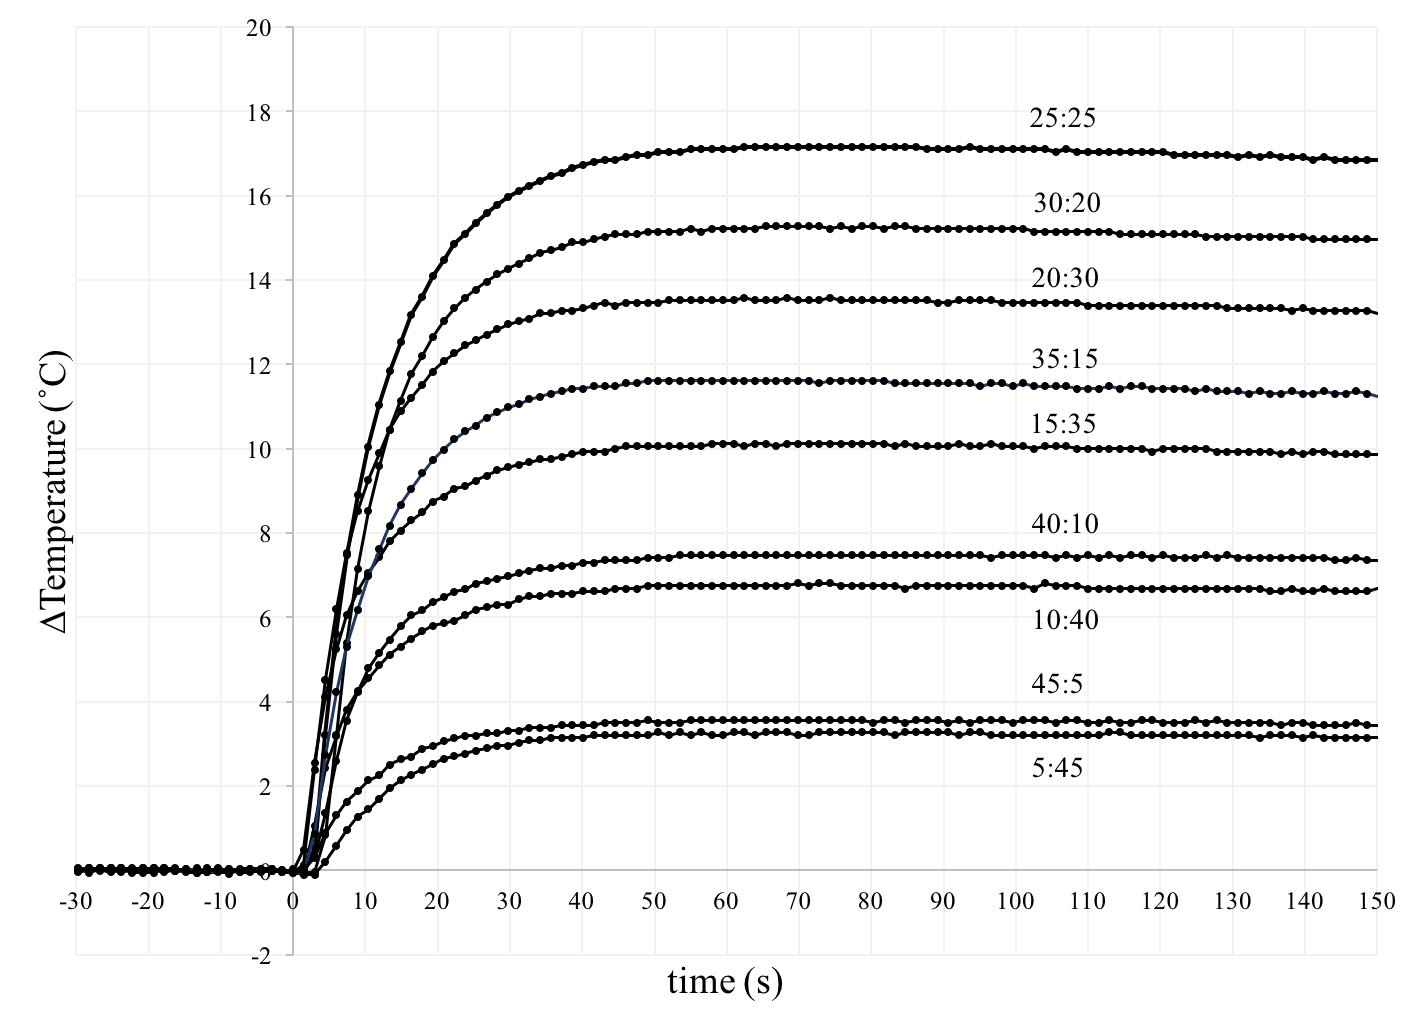
\includegraphics[width=\textwidth]{Temperature_Profiles_Na2SO3_BW.png}
\caption{Variation of Temperature with Time for Mixtures of NaClO($aq$) and Na$_2$SO$_3$($aq$)}
\label{fig:temp_Na2SO3}
\end{figure}

The maximum $\Delta T$ for each mixture was recorded and plotted 
against the volume of NaClO($aq$) in the mixture; these results are shown in Figure~\ref{fig:var_Na2SO3}.  
Points corresponding to 0.0 mL NaClO($aq$):50.0 mL Na$_2$SO$_3$($aq$) and 50.0 mL NaClO($aq$):0.0 mL Na$_2$SO$_3$($aq$) 
(each with $\Delta T_\mathrm{max} = 0.0^\circ$C) were included.  Lines of best fit were generated through each the upward and downward 
trends.\footnote{The point corresponding to 25.0 mL NaClO($aq$):25.0 mL Na$_2$SO$_3$($aq$) was included in the upward trend.  
As before, the lines were forced through the end points.  The resulting equations of the lines of best fit 
are: $\Delta T_\mathrm{max}$ = (0.6813$^\circ$C/mL) $V$ ($R^2$ = 0.99977) and $\Delta T_\mathrm{max}$ = ($-0.7629^\circ$C/mL) $V$ + 38.145$^\circ$C ($R^2$= 0.99923).}  
The intersection of these lines occurs at 26.4 mL NaClO($aq$) and $\Delta T_\mathrm{max} = 18.0^\circ$C.  This 
corresponds to a predicted optimal ratio of 26.4 mL NaClO($aq$) to 23.6 mL Na$_2$SO$_3$ (simplified to 1.12:1), 
which is in agreement with the predicted stoichiometry of 1:1.\footnote{The actual stoichiometry of 1:1 is 
based on the net ionic equation: ClO$^-$($aq$) + SO$_3^{2-}$($aq$) $\rightarrow$ Cl$^-$($aq$) + SO$_4^{2-}$($aq$)~\cite{vonderbrink}.}

\begin{figure}[htbp]
\centering
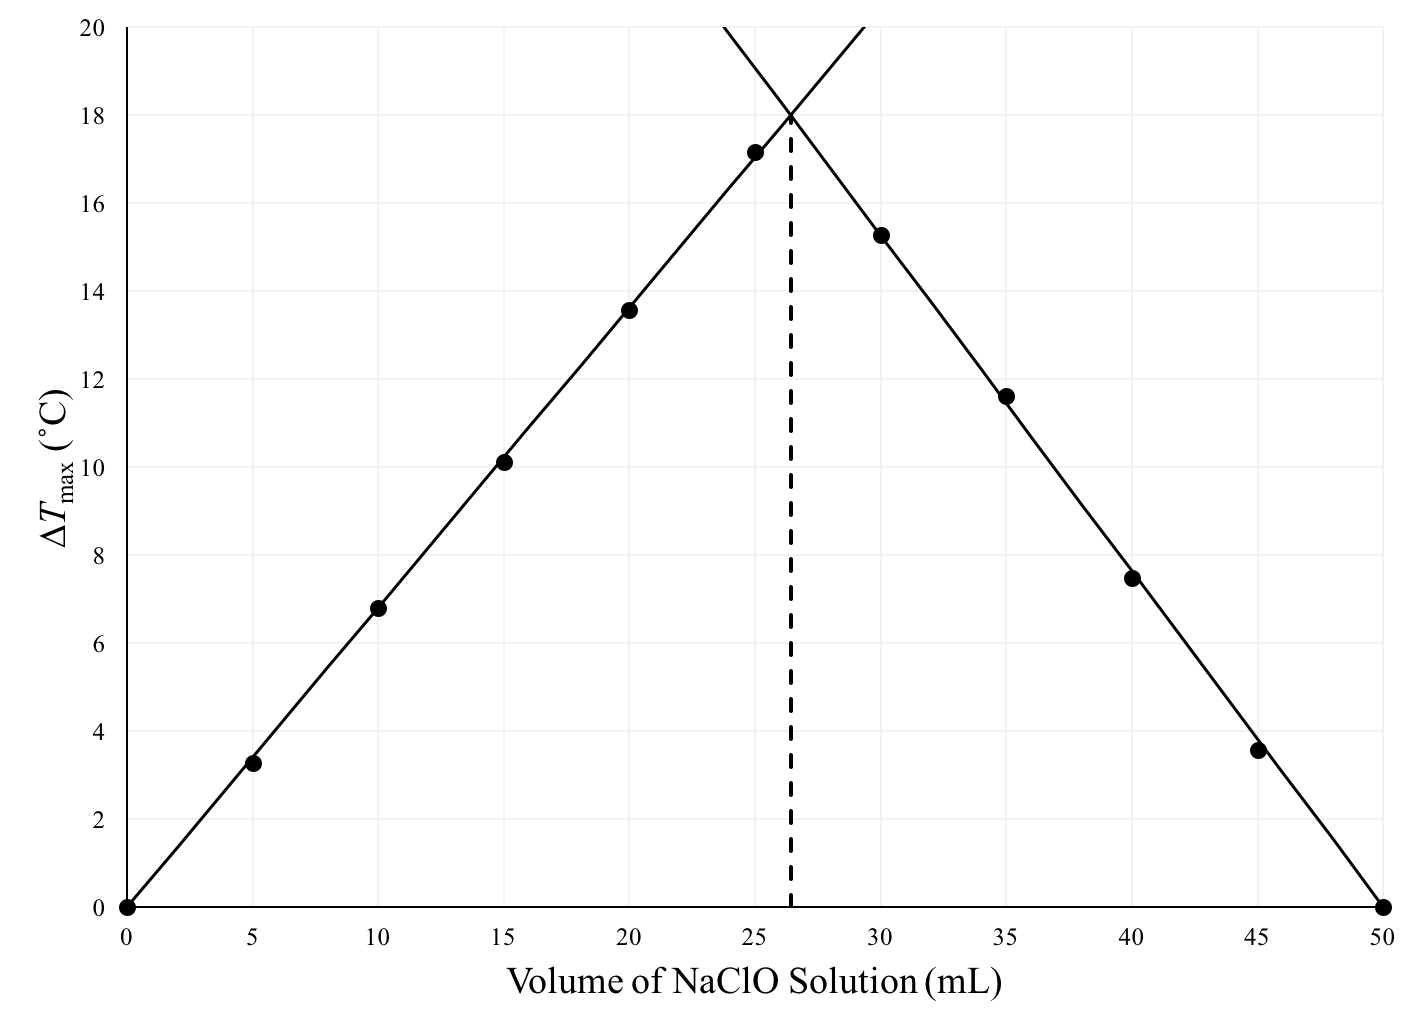
\includegraphics[width=\textwidth]{Bleach_Na2SO3_Variations.png}
\caption{Maximum Temperature Changes Observed for Each Reaction Mixture of NaClO($aq$) and Na$_2$SO$_3$($aq$)}   %Variation of Temperature with Time for Mixtures of NaClO($aq$) and KI($aq$)}
\label{fig:var_Na2SO3}
\end{figure}

\subsection{Improving the Accuracy of Results}
The method employed above allows students to quickly and easily determine the stoichiometric ratio in a chemical reaction with minimal calculations.  
The determined ratios of 3.17:1 (NaClO:KI) and 1.12:1 NaClO:Na$_2$SO$_3$ were of sufficient accuracy to conclude the correct ratios of 3:1 and 1:1 when 
rounded to the nearest whole number.  The accuracy of these ratios can be improved using some post-lab corrections.  One notable correction involves the 
adjustment of the initial temperature.  Initial temperature was determined using only the component in the mixture with the largest volume; this 
assumes that both reactants are at this initial temperature.  If the components are at different initial temperatures, a weighted average can be 
utilized~\cite{vonderbrink} to determine a more representative initial temperature as:
\begin{displaymath}
T_{i,\mathrm{avg}} = \left(\frac{V_\mathrm{A}}{V}\right)T_{i,\mathrm{A}} + \left(\frac{V_\mathrm{B}}{V}\right)T_{i,\mathrm{B}}
\end{displaymath}
where $V_\mathrm{A}$ and $V_\mathrm{B}$ represent the volumes of components A and B in the mixture, $V$ represents the total volume of the mixture, 
and $T_{i,\mathrm{A}}$ and $T_{i,\mathrm{B}}$ represent the initial temperatures of components A and B.\footnote{In order to apply this correction, 
an additional measurement of the initial temperature of the minor component must be obtained using a separate thermometer.}  This temperature 
correction was applied to the NaClO/Na$_2$SO$_3$ reactions; results are shown in Figure~\ref{fig:var_Na2SO3_corr}.\footnote{When conducting the 
experiment using these reactants, initial temperatures varied by as much as 2$^\circ$C.  Initial temperature variations for the NaClO/KI reactions 
were less significant at approximately $0.5^\circ$C.} 

\begin{figure}[htbp]
\centering
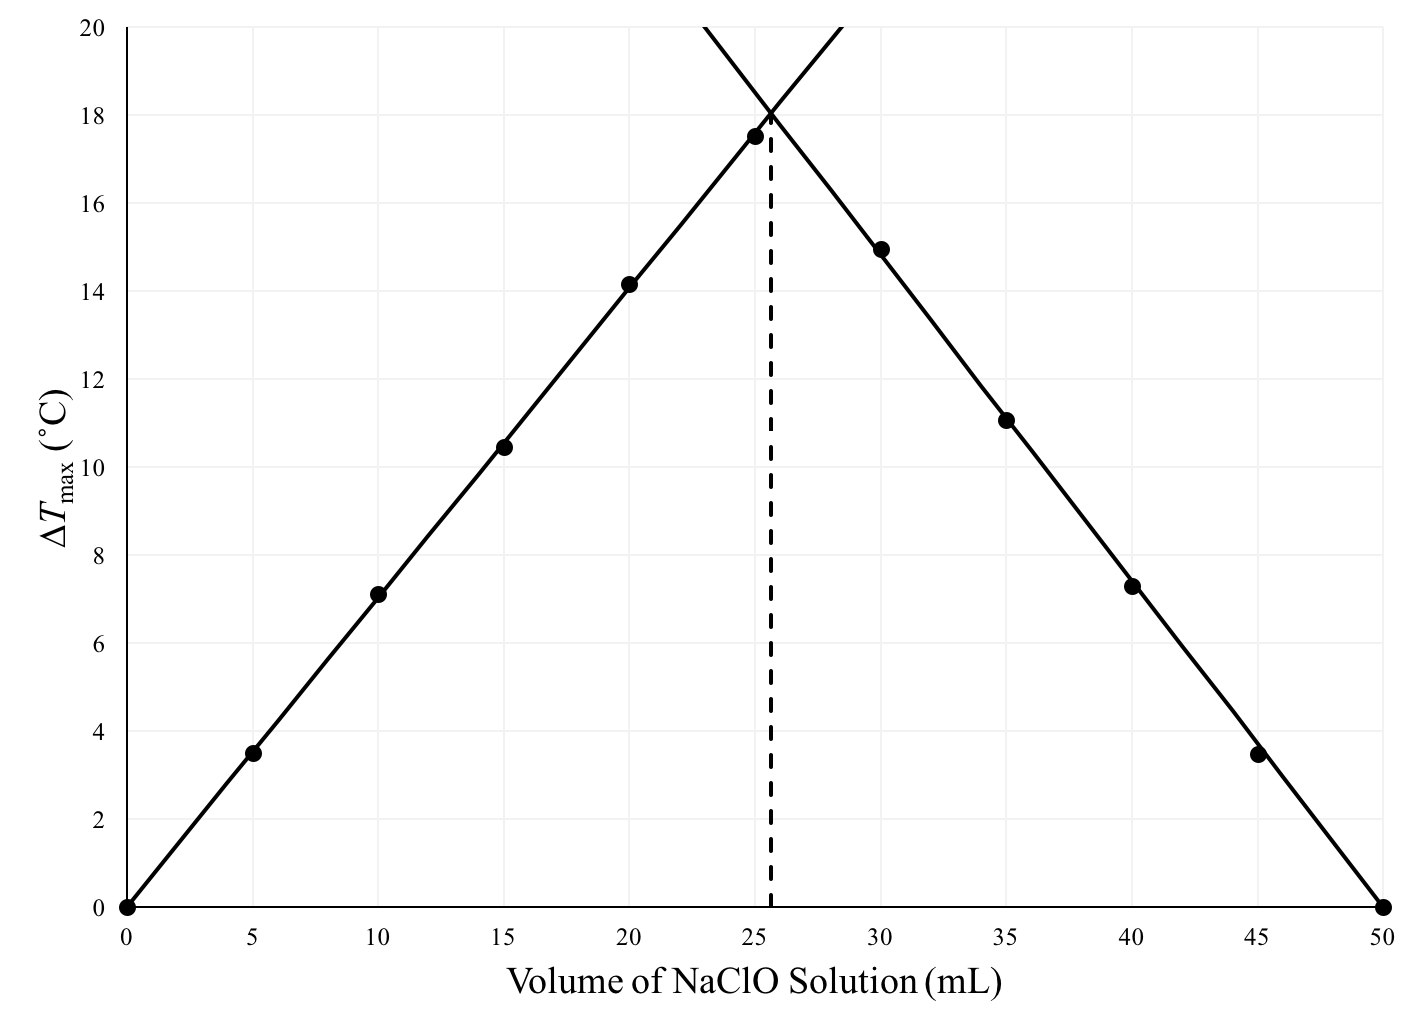
\includegraphics[width=\textwidth]{Bleach_Na2SO3_Variations_Corrected.png}
\caption{Maximum Temperature Changes for Mixtures of NaClO($aq$) and Na$_2$SO$_3$($aq$) with Initial Temperature Correction}   %Variation of Temperature with Time for Mixtures of NaClO($aq$) and KI($aq$)}
\label{fig:var_Na2SO3_corr}
\end{figure}

The corrected data yield a more accurate ratio of 25.6 mL NaClO(aq) to 24.4 mL Na$_2$SO$_3$($aq$), 
which simplifies to 1.05:1.  The observed variations are also more symmetric about the intersection composition, as is expected for a 1:1 ratio.  

The method used assumes equal concentrations of the reactants.  Slight differences in concentrations may lead to deviations from the true ratios.  
Concentrations can be incorporated using the expression
\begin{displaymath}
\mathrm{Ratio} = \frac{n_\mathrm{A}}{n_\mathrm{B}} = \frac{M_\mathrm{A}V_\mathrm{A}}{M_\mathrm{B}V_\mathrm{B}}
\end{displaymath}
where $M$ represents the molar concentration of component A or B, $V$ represents the volume of A or B at the optimal ratio, and $n$ indicates the amount
of the component A or B at the optimal ratio.  
This can be an important correction if the NaClO($aq$) solution was prepared from an older bleach solution, as some decomposition is possible.  An accurate 
concentration of NaClO($aq$) can be determined through titration analysis~\cite{vonderbrink}.  

